\documentclass{article}
\usepackage{amsmath}
\usepackage{amssymb}
\usepackage{graphicx}
\usepackage[margin=1in]{geometry}
\usepackage{hyperref}
\usepackage{caption}
\usepackage{float}
\graphicspath{{images/}}
\hypersetup{
    colorlinks=true,
    urlcolor=blue,
}
\begin{document}

\title{Rendering zonotope cross-sections}
\author{Aresh Pourkavoos}
\maketitle

This project is the culmination of a train of thought
that started around a year ago
with the question of whether I could build an icosahedron in Minecraft.
I had learned that the coordinates of its vertices
were based on the golden ratio $\varphi = \frac{1+\sqrt{5}}{2}$,
the positive solution to the equation $\varphi^2 = \varphi+1$.
More specifically,
an icosahedron can be constructed with three mutually perpendicular golden rectangles:

\begin{center}
  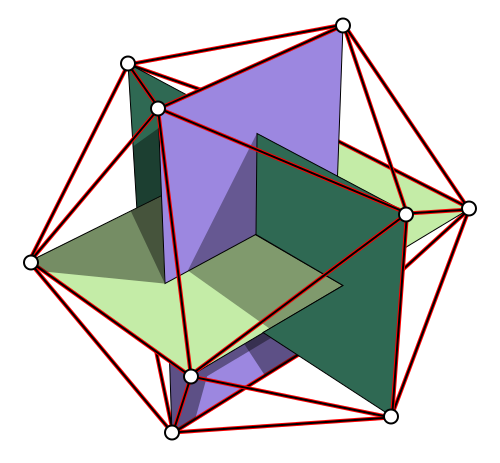
\includegraphics[width=0.25\linewidth]{rects.png}\\
  (Source: Wikimedia Commons)
\end{center}

If the icosahedron has a side length of 2,
then the rectangles are $2 \times 2\varphi$,
and the coordinates of their vertices are
\[
(0, \pm 1, \pm \varphi),
(\pm 1, \pm \varphi, 0),
(\pm \varphi, 0, \pm 1).
\]
More succinctly, the coordinate are formed from all permutations and sign changes of
\[(0, 1, \varphi).\]
Since $\varphi$ is irrational,
there is no way to scale these coordinates
such that they fall exactly on integers.
(For the readers who are considering rotations,
the proof that they don't work either is left as an exercise.)
However, it is possible to approximate it using the Fibonacci numbers,
since they obey the same ``power law'' as $\varphi$,
i.e. $\varphi^{n}+\varphi^{n+1}=\varphi^{n+2}$ and $F_n+F_{n+1}=F_{n+2}$.
(Define $F_0=0$ and $F_1=1$.)
For this reason, the ratio of consecutive Fibonacci numbers approaches $\varphi$,
so we may approximate the coordinates of an icosahedron with
\[(0, F_n, F_{n+1})\]
for some $n$,
e.g. (0, 3, 5) for $n=4$.
Placed into Minecraft, the vertices and the golden rectangles joining them look like this:

\begin{center}
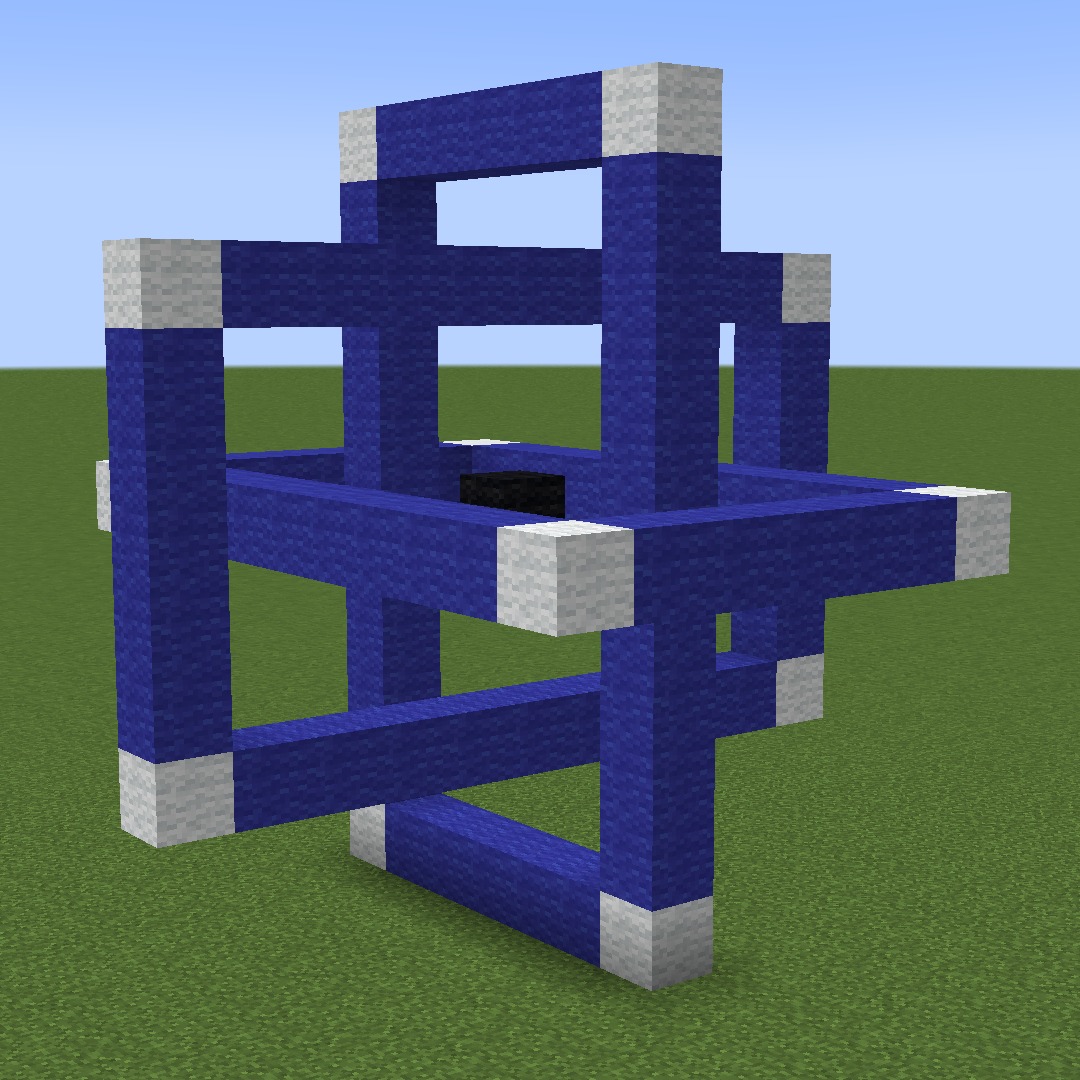
\includegraphics[width=0.25\linewidth]{ike.png}
\end{center}

But how do we fill in the edges?
Some of them are just the short edges of the rectangles,
so a straight line of blocks will suffice.
However, these only account for 6 of the 30 edges,
where the other 24 join vertices between different rectangles.
For the example above,
all of these are permutations and sign changes of
\[(5, 3, 2).\]
In the general Fibonacci case,
they would be $(F_{n+1}, F_n, F_{n-1})$,
and in the exact case,
they would be \\$(\varphi, 1, \varphi-1)$.
So how do we fill such a line with blocks
in a continuous and ``voxel-perfect'' way?

Before defining a voxel-perfect line in 3D,
it is beneficial to define a pixel-perfect line in 2D.
Suppose without loss of generality
that it is drawn between $(0, 0)$ and $(x, y)$,
where $x$ and $y$ are integers and $0 \leq x \leq y$.
(All other lines may be created by reflecting across
the $x$-axis, the $y$-axis, the line $y=x$,
or some combination of these,
which are all well-defined at the pixel level.)
To make it pixel-perfect,
exactly $y+1$ pixels must be filled in (including both endpoints),
one in each $y$-coordinate.
For a given $y$-coordinate,
the center of the pixel is decided
by connecting the centers of the endpoints,
intersecting this line with the appropriate row,
and filling the pixel whose center lies closest to this intersection.
A pixel-perfect line where $x=3$ and $y=5$ is shown below.

\begin{center}
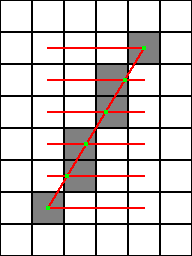
\includegraphics[width=0.25\linewidth]{grid1.png}
\end{center}

If there is a tie in the rounding, \textit{no} pixel-perfect line exists,
since it could not be symmetric without adding an extra pixel in the center
or creating a gap in the line.
This situation occurs whenever $x$ is odd and $y$ is even,
or in general, when the smaller coordinate is odd and the larger is even.
For example, $x=3$ and $y=4$ has no pixel-perfect line as shown below,
where the cells with ambiguous filling are striped.

\begin{center}
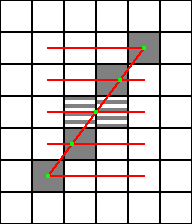
\includegraphics[width=0.25\linewidth]{grid2.png}
\end{center}

Finally, if $x$ and $y$ share a common factor $k$,
any line with vector $(x, y)$
is just $k$ copies of the line $\left(\frac{x}{k}, \frac{y}{k}\right)$
connected end-to-end.
The pixel-perfection of the overall line
depends exactly on the pixel-perfection of these smaller copies.
Together, these facts characterize exactly which lines are pixel-perfect.

Before moving on to voxel-perfection,
consider drawing lines from the origin to $(F_n, F_{n+1})$
for some $n \geq 0$.
This could be used to draw lines in 3D from the center of an icosahedron to its vertices,
since the third coordinate is 0.
It is relatively easy to prove that consecutive Fibonacci numbers have no common factors,
so all that matters is whether $F_n$ and $F_{n+1}$ are even or odd.
As the table below shows,
$F_n$ is even for all $n$ which are multiples of 3
and odd for all other $n$.
$F_n \leq F_{n+1}$,
so $F_{n+1}$ may be treated as $y$.
If $n+1$ is a multiple of 3, then $F_{n+1}$ is even and $F_n$ is odd,
so no pixel-perfect line exists.
Otherwise, $F_{n+1}$ is odd, so there is no problem drawing a pixel-perfect line.

\begin{center}
\begin{tabular}{|c|c|c|c|c|c|c|}
  \hline
  $n$ & 0 & 1 & 2 & 3 & 4 & 5 \\ \hline
  $F_n$ & 0 & 1 & 1 & 2 & 3 & 5 \\ \hline
  $F_n \mod 2$ & 0 & 1 & 1 & 0 & 1 & 1 \\ \hline
  $F_{n+1}$ & 1 & 1 & 2 & 3 & 5 & 8 \\ \hline
  $F_{n+1} \mod 2$ & 1 & 1 & 0 & 1 & 1 & 0 \\ \hline
  Possible? & Yes & Yes & No & Yes & Yes & No \\ \hline
\end{tabular}
\end{center}

For voxel-perfection, the situation is similar.
The line should only be one voxel thick,
so the coordinate with the largest change needs to be identified
(say $0 \leq x \leq y \leq z$),
and only one voxel should be filled in 
per $z$-coordinate between and including the endpoints
for a total of $z+1$ voxels.
Each filled-in voxel is found by intersecting the (exact) line between the endpoints
with the $z+1$ different planes and rounding the coordinates to the nearest voxel.
This is equivalent to finding pixel-perfect lines for vectors of $(x, z)$ and $(y, z)$
and combining the $x$- and $y$-coordinates for the pixels on each line.

Now we can find out whether the rest of the icosahedron's edges can be filled in.
For the specific case of $(5, 3, 2)$ edges,
$(5, 3)$ and $(5, 2)$ both have pixel-perfect lines,
so the full wireframe can be built out of voxels:

\begin{center}
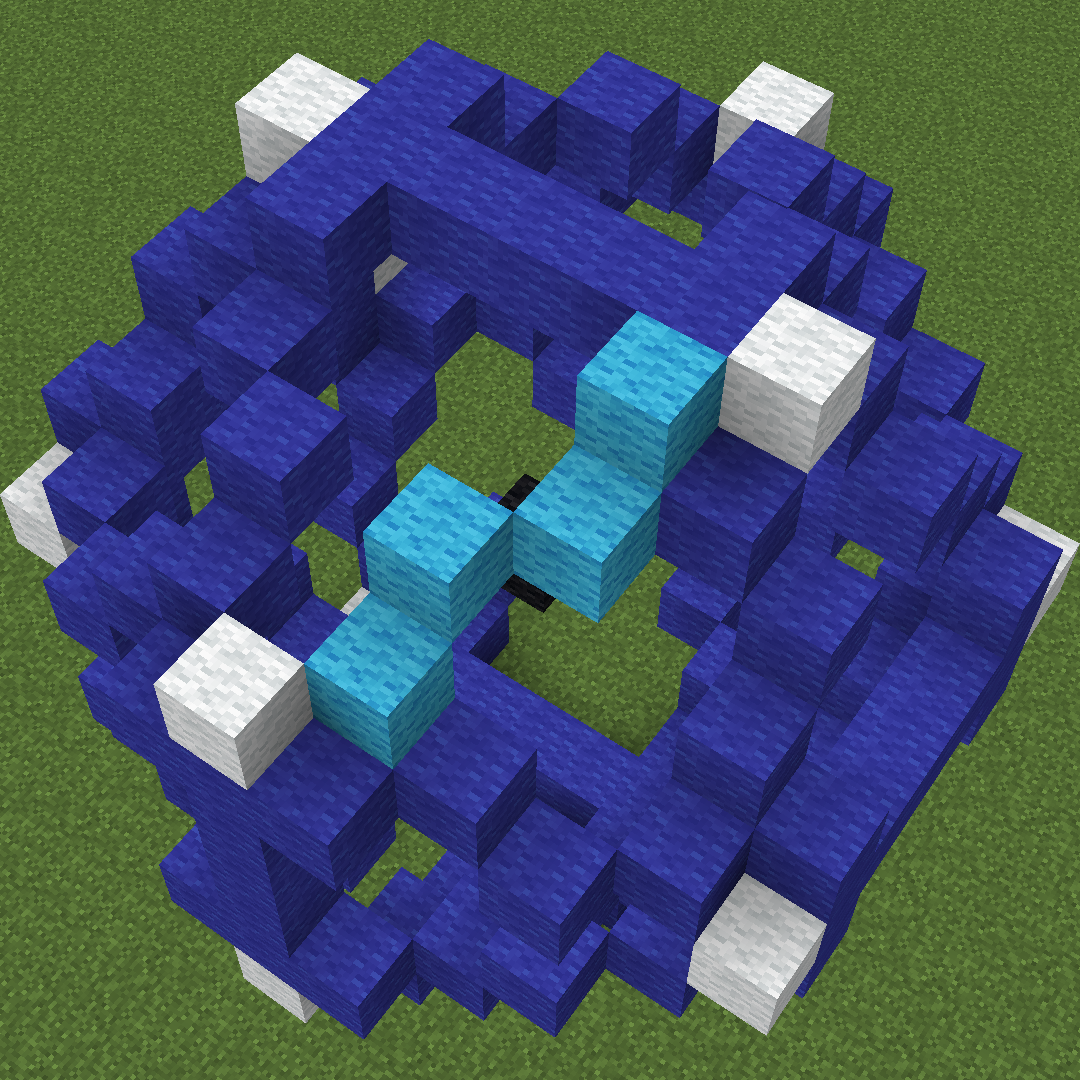
\includegraphics[width=0.25\linewidth]{ike2.png}
\end{center}

This icosahedron is viewed edge-first, with the foremost edge highlighted in light blue.
Viewing this edge along 2 out of the 3 axes will result in
the pixel-perfect lines for $(5, 3)$ and $(5, 2)$,
and the third axis creates thicker, non-pixel-perfect line for $(3, 2)$.
In the general case, the icosahedron's edge is $(F_{n+1}, F_n, F_{n-1})$,
and it can be made voxel-perfect if and only if
$(F_{n+1}, F_n)$ and $(F_{n+1}, F_{n-1})$ can both be made pixel-perfect.
Since, $F_{n+1}$ and $F_n$ are coprime as before,
so are $F_{n+1}$ and $F_{n-1}$, since $F_{n-1}=F_{n+1}-F_n$.
It also may be seen from the table that the same conditions on $n$ apply as before,
i.e. the line is voxel-perfect exactly when $n+1$ is not a multiple of 3.
So out of all possible ways to scale this icosahedron by a power of $\varphi$,
every third one does not allow for voxel-perfect lines.
Moving in the $z$-direction along one of these lines,
the $x$- and $y$-coordinates of the voxel increment in a pattern
which is aperiodic as $n$ increases,
characterized by
\href{https://oeis.org/A334414}{OEIS sequence A334414}.

With this system in hand, I was able to build other shapes with icosahedral symmetry,
including rhombic triacontahedra:

\begin{center}
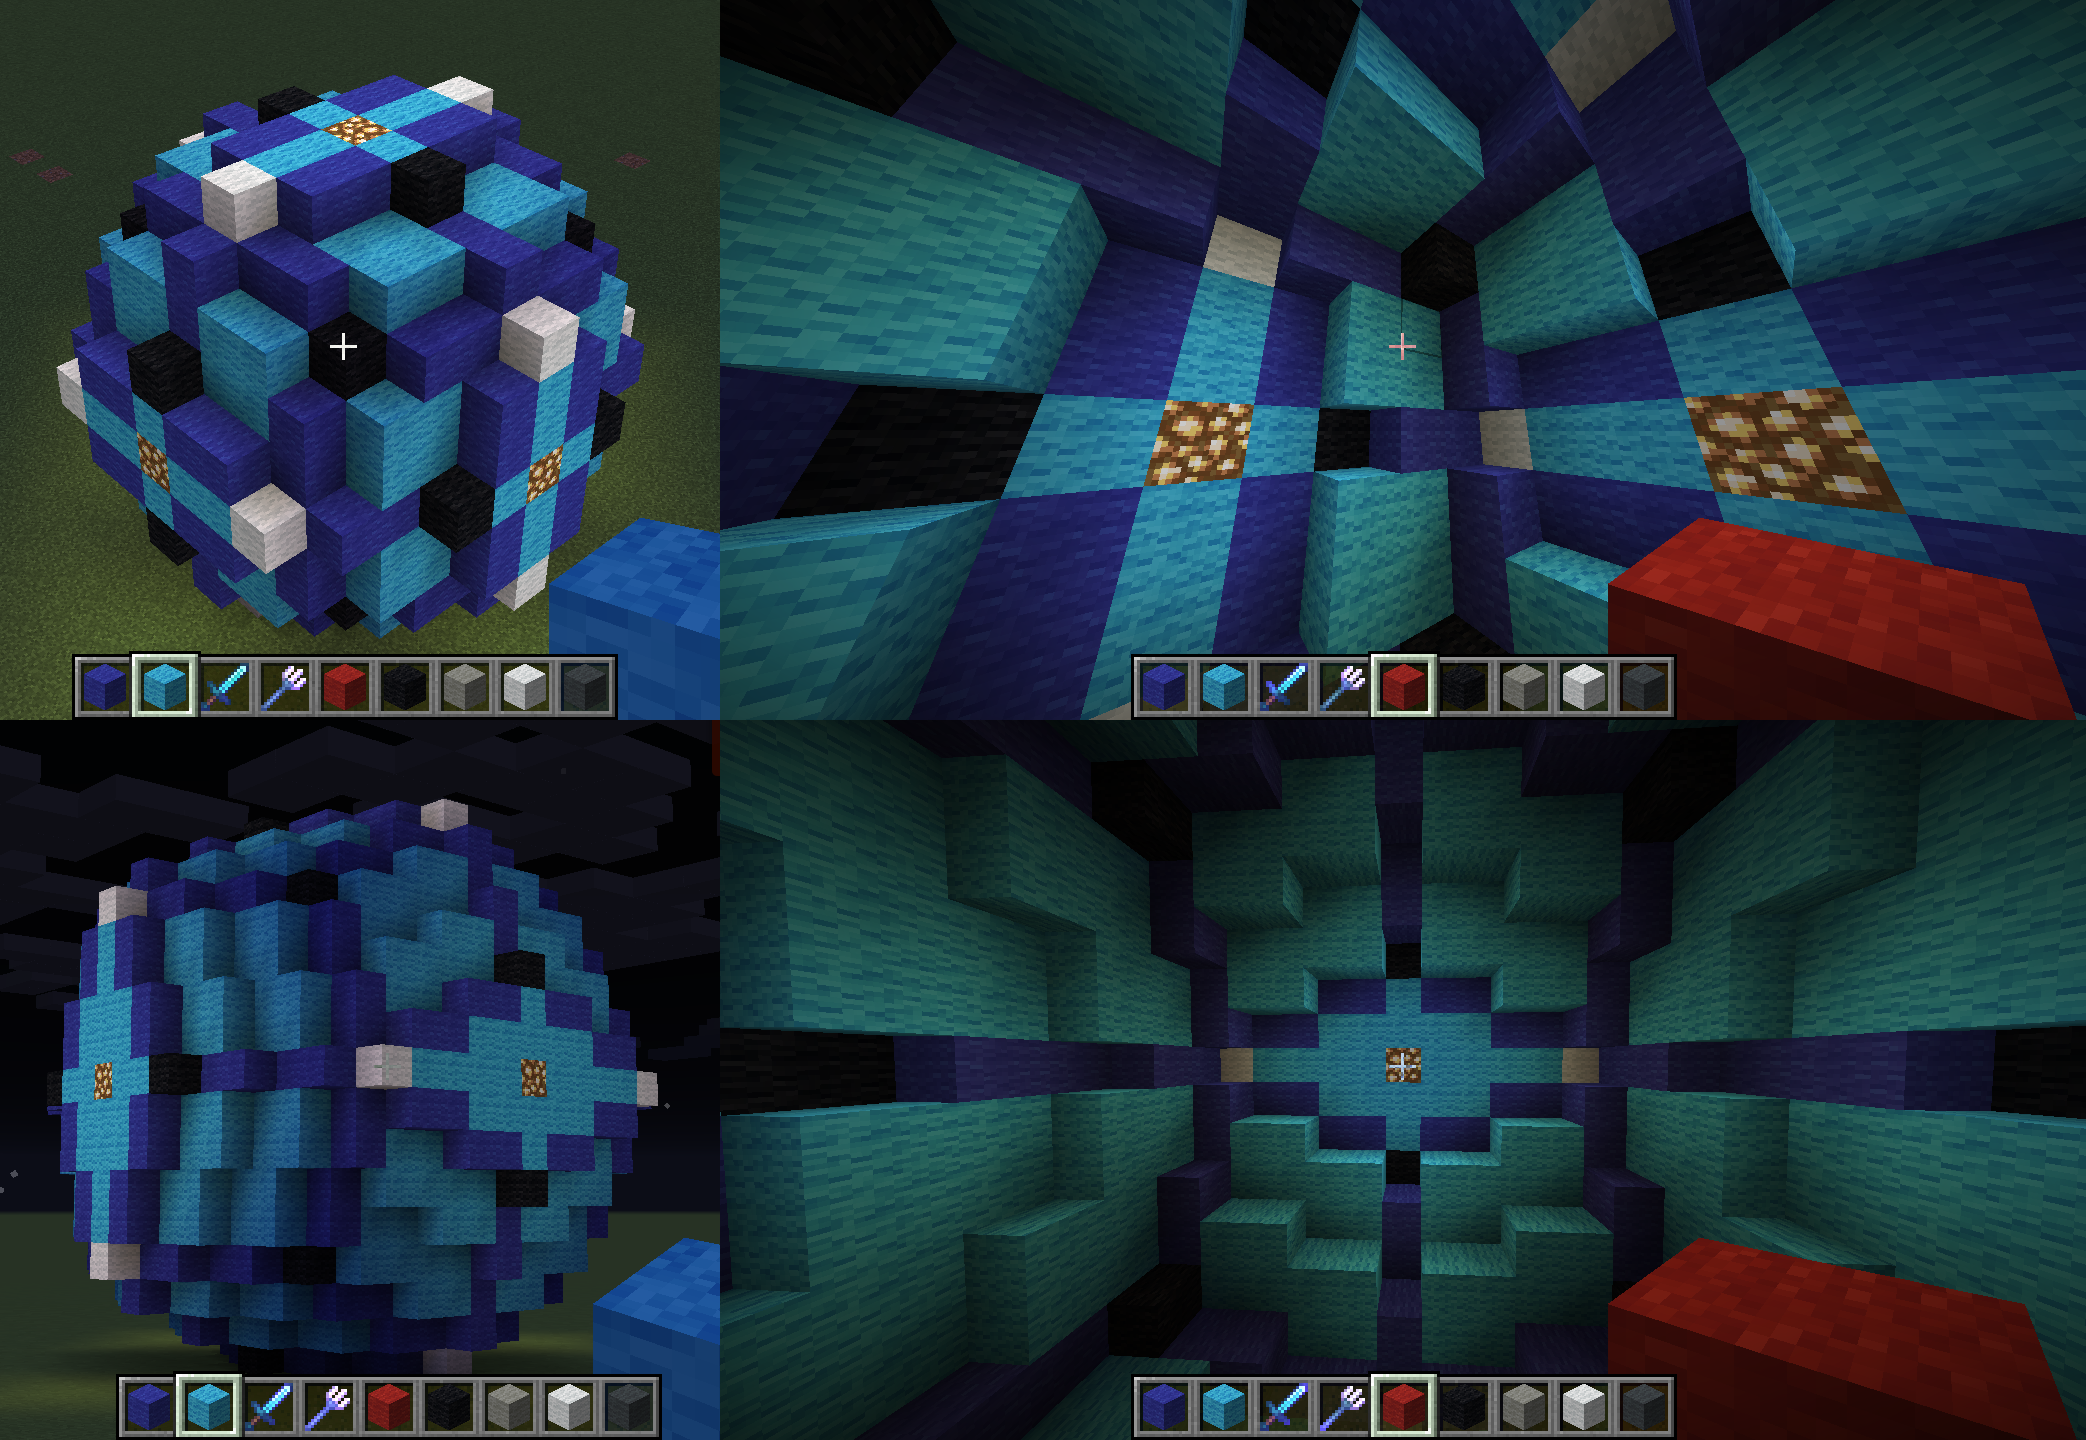
\includegraphics[width=\linewidth]{tria.png}
\end{center}

But why stop at 3 dimensions?
There are many 4D shapes (polychora) which also have coordinates based on the golden ratio.
However, since 4D voxel building games are somewhat hard to come by,
I had to resort to programming to generate them.
Since it's difficult to input every vertex and edge manually,
I turned to a subset of these objects which could be generated using a very different approach:
the Minkowski sum.

The Minkowski sum is a way to combine two point sets to create another,
potentially of a higher dimension.
It works by adding the coordinates of each point in one set
to those of each point in the other.
For example, the image below shows how
the Minkowski sum of two perpendicular line segments of equal length (dark gray)
is a square (light gray),
where the red lines are drawn between the origin (black),
a point on each segment, and their sum.
\begin{center}
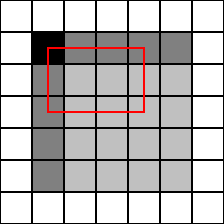
\includegraphics[width=0.25\linewidth]{mink.png}
\end{center}
Taking the Minkowski sum with more perpendicular line segments of equal length
creates cubes in higher dimensions.
However, these segments do not have to be either of these,
and in general, the shapes that can be formed are known as \textit{zonotopes}.
One such polychoron with golden-ratio coordinates is the omnitruncated 120-cell,
whose projection into 3 dimensions is shown:
\begin{center}
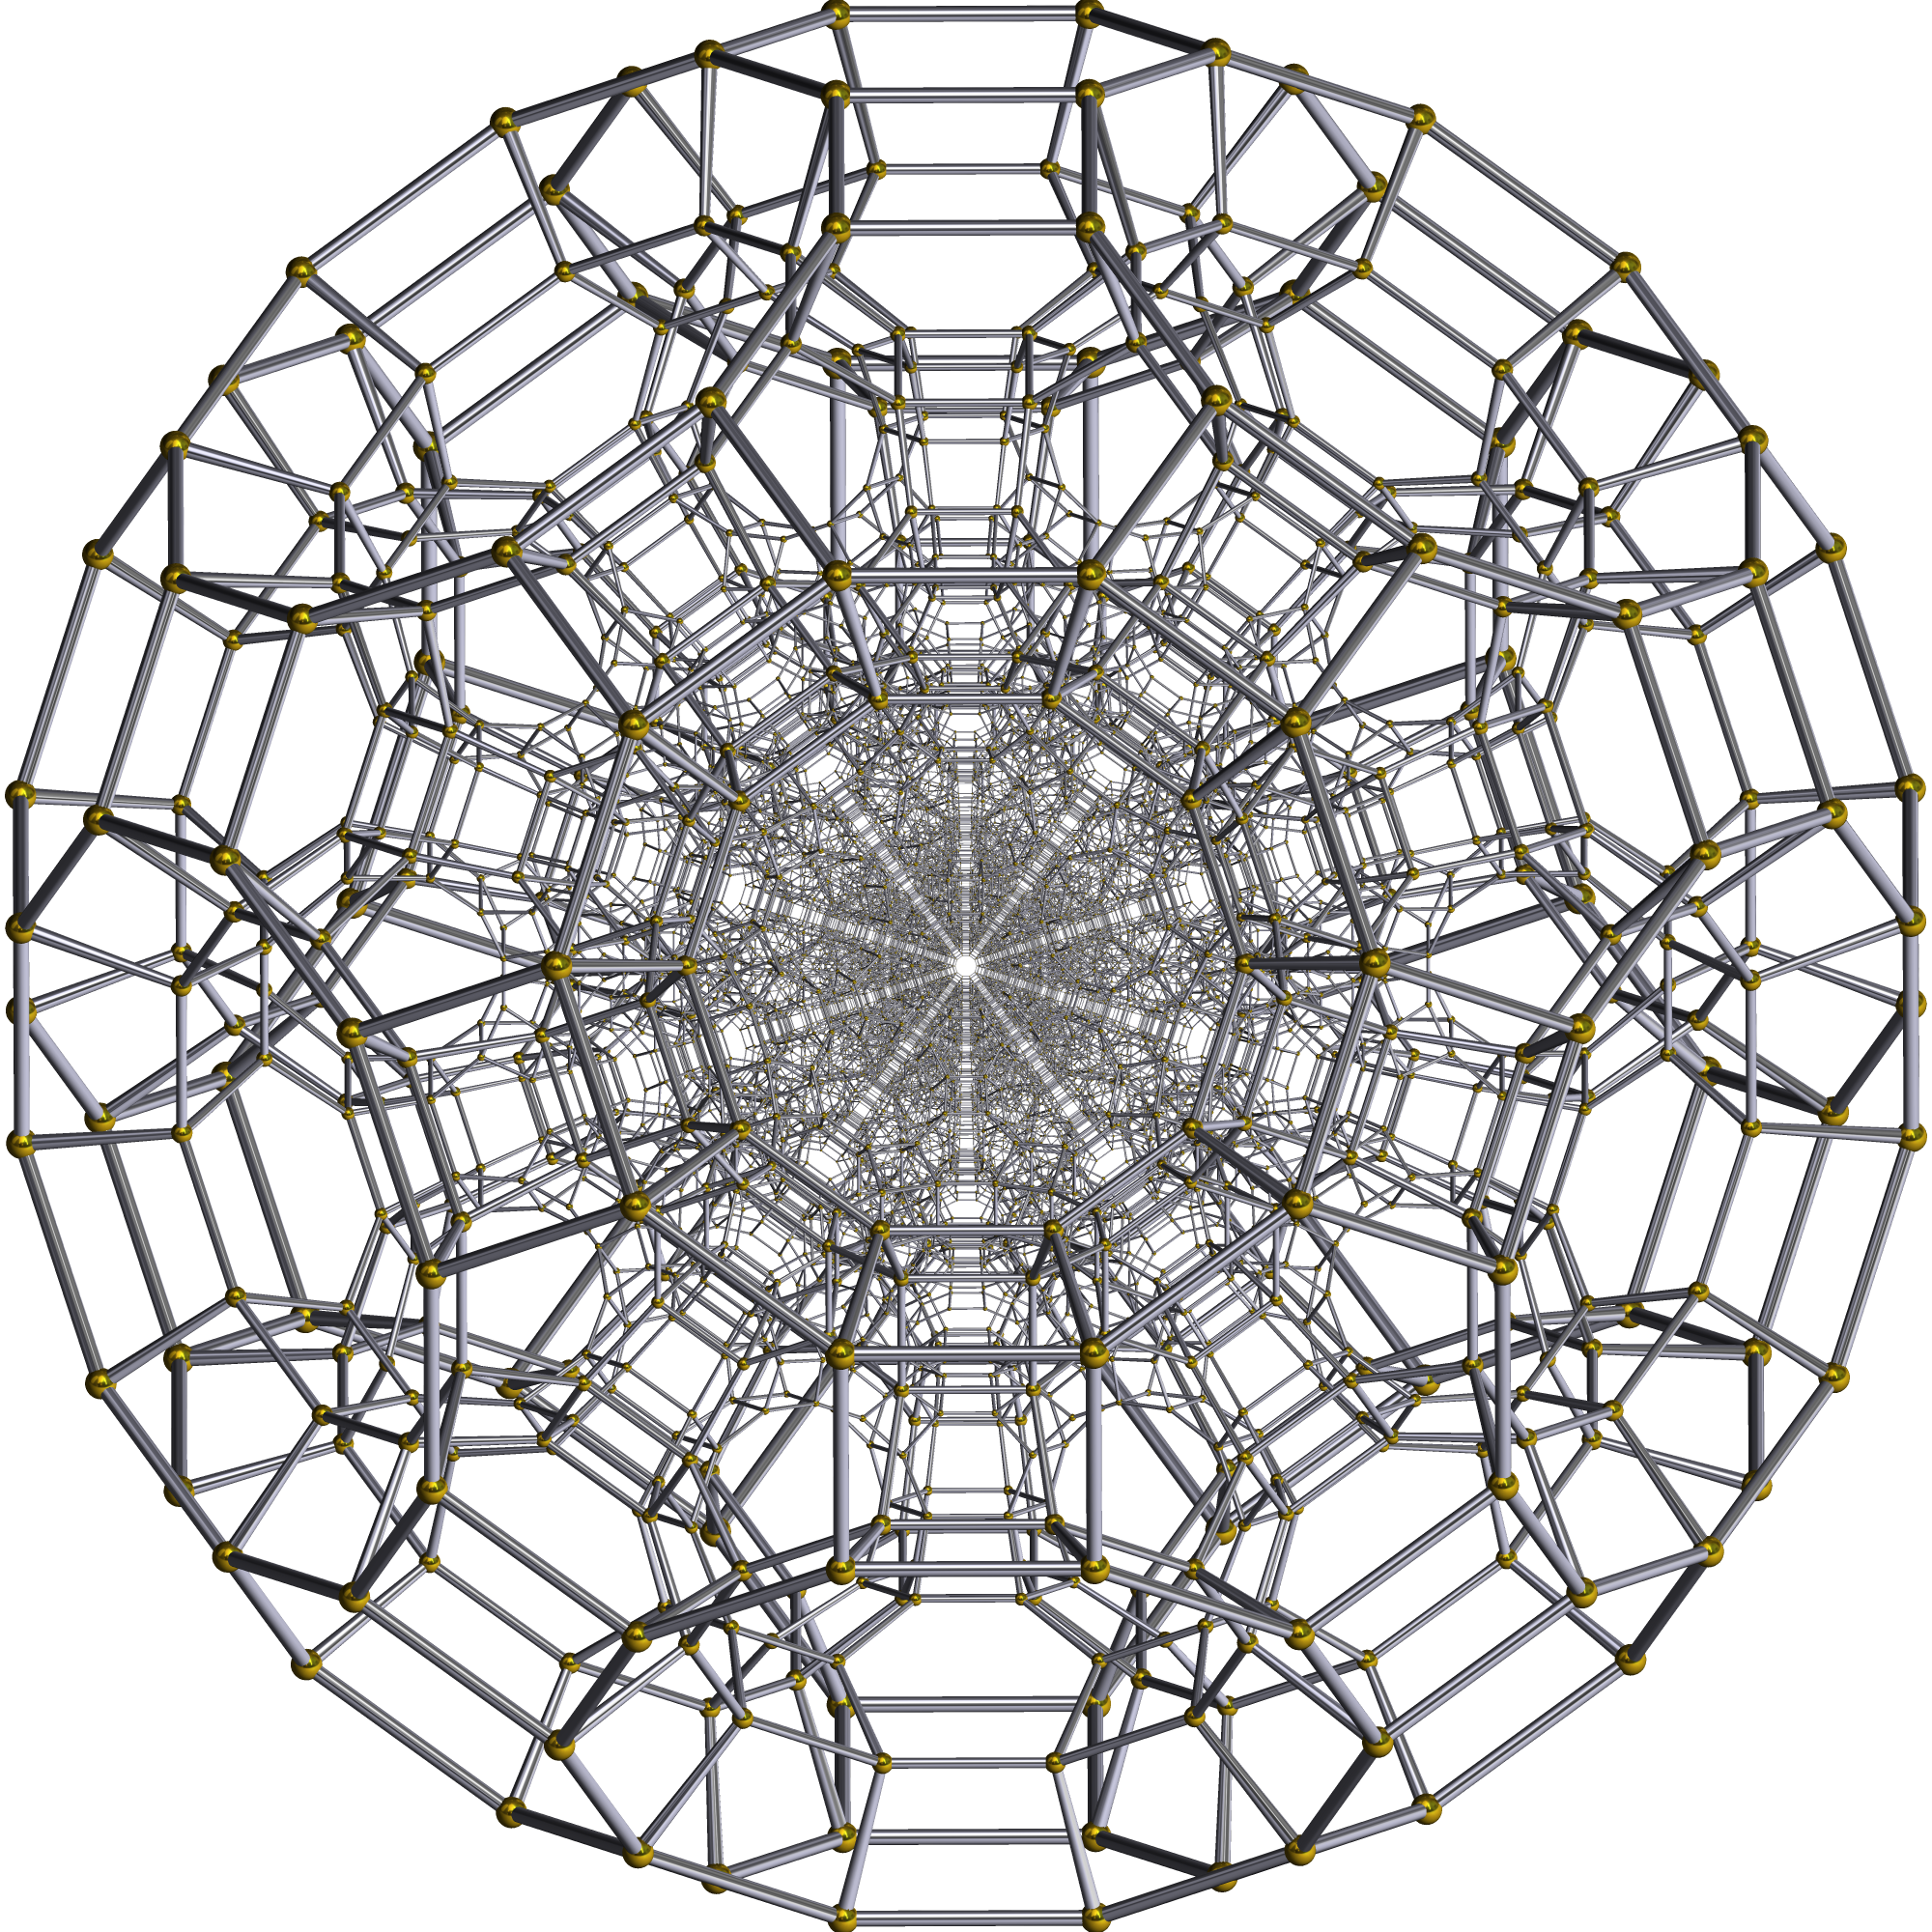
\includegraphics[width=0.5\linewidth]{gidpixhi.png}\\
(Made with \href{http://www.software3d.com/Stella.php}{Stella4D})
\end{center}
It may be constructed as a Minkowski sum of the line segments
connecting the origin to the vertices of the 600-cell,
a simpler polychoron with the same symmetry.
All I had to do then was to construct the ``hypervoxel-perfect'' approximations of these segments
and write a C program to take their Minkowski sum.
However, I also wanted to color the outside of this polychoron
based on its cells, or 3D ``faces.''
Fortunately, all elements of a zonotope are also zonotopes,
so I had to find which segments to sum to create each cell,
as well as the offset necessary to put it in the right place.
Since the omnitruncated 120-cell has 2640 cells,
there was no way I was going to hand-code the set of segments for each one.

Instead, I found the normal vector to each cell,
a much less tedious process since most are formed by permutations,
and then take the dot product of each line segment and the vector.
If the dot product is 0, the segment lies flat on the cell and should be used in the sum.
If it is positive, the segment points in the direction of the cell
and should contribue to the offset.
If negative, the line segment is ignored.
It took some optimization to run in a reasonable amount of time,
since I was dealing with arrays of over 80 million hypervoxels,
but I eventually had a program that spat out an ASCII-art version of the omnitruncated 120-cell,
one 2D cross section at a time.
I then had to write a Processing sketch to render the GIFs which are not embedded in this PDF
but located in the ``images'' directory.
The programming side of things may be explained in a later entry.

\end{document}
